
%% bare_conf.tex
%% V1.4b
%% 2015/08/26
%% by Michael Shell
%% See:
%% http://www.michaelshell.org/
%% for current contact information.
%%
%% This is a skeleton file demonstrating the use of IEEEtran.cls
%% (requires IEEEtran.cls version 1.8b or later) with an IEEE
%% conference paper.
%%
%% Support sites:
%% http://www.michaelshell.org/tex/ieeetran/
%% http://www.ctan.org/pkg/ieeetran
%% and
%% http://www.ieee.org/

%%*************************************************************************
%% Legal Notice:
%% This code is offered as-is without any warranty either expressed or
%% implied; without even the implied warranty of MERCHANTABILITY or
%% FITNESS FOR A PARTICULAR PURPOSE! 
%% User assumes all risk.
%% In no event shall the IEEE or any contributor to this code be liable for
%% any damages or losses, including, but not limited to, incidental,
%% consequential, or any other damages, resulting from the use or misuse
%% of any information contained here.
%%
%% All comments are the opinions of their respective authors and are not
%% necessarily endorsed by the IEEE.
%%
%% This work is distributed under the LaTeX Project Public License (LPPL)
%% ( http://www.latex-project.org/ ) version 1.3, and may be freely used,
%% distributed and modified. A copy of the LPPL, version 1.3, is included
%% in the base LaTeX documentation of all distributions of LaTeX released
%% 2003/12/01 or later.
%% Retain all contribution notices and credits.
%% ** Modified files should be clearly indicated as such, including  **
%% ** renaming them and changing author support contact information. **
%%*************************************************************************


% *** Authors should verify (and, if needed, correct) their LaTeX system  ***
% *** with the testflow diagnostic prior to trusting their LaTeX platform ***
% *** with production work. The IEEE's font choices and paper sizes can   ***
% *** trigger bugs that do not appear when using other class files.       ***                          ***
% The testflow support page is at:
% http://www.michaelshell.org/tex/testflow/



\documentclass[conference]{IEEEtran}
\usepackage{graphicx}
\usepackage[utf8]{inputenc}
\usepackage[T1]{fontenc} 
%\usepackage[latin1]{inputenc}
\usepackage{pifont} 
\usepackage{import}
\usepackage{amsmath}
\usepackage{multirow}
\usepackage{graphicx,url}
\usepackage{placeins}
\usepackage{adjustbox}
\usepackage[english]{babel}
\usepackage{lipsum}
\usepackage{multicol}
\usepackage{textcomp}
\usepackage{listings}
\usepackage[svgnames]{xcolor} 
\usepackage{caption}
\usepackage{amsmath}
\usepackage{calc} 
\usepackage{array,url,kantlipsum}
\usepackage{algorithm}
\usepackage{algpseudocode}
\usepackage{lscape}
\usepackage{array}
\usepackage{longtable}
\usepackage{booktabs}
\usepackage{txfonts}
\usepackage{colortbl}%
  \newcommand{\myrowcolour}{\rowcolor[gray]{0.925}}
\newenvironment{Figure}
  {\par\medskip\noindent\minipage{\linewidth}}
  {\endminipage\par\medskip}
  
\lstset{
language=Java,
basicstyle=\small\ttfamily,
numbers=left,
numbersep=5pt,
xleftmargin=20pt,
frame=tb,
framexleftmargin=20pt
}

\renewcommand*\thelstnumber{\arabic{lstnumber}:}

\DeclareCaptionFormat{mylst}{\hrule#1#2#3}
\captionsetup[lstlisting]{format=mylst,labelfont=bf,singlelinecheck=off,labelsep=space,font={normalsize,tt}}




% Some Computer Society conferences also require the compsoc mode option,
% but others use the standard conference format.
%
% If IEEEtran.cls has not been installed into the LaTeX system files,
% manually specify the path to it like:
% \documentclass[conference]{../sty/IEEEtran}





% Some very useful LaTeX packages include:
% (uncomment the ones you want to load)


% *** MISC UTILITY PACKAGES ***
%
%\usepackage{ifpdf}
% Heiko Oberdiek's ifpdf.sty is very useful if you need conditional
% compilation based on whether the output is pdf or dvi.
% usage:
% \ifpdf
%   % pdf code
% \else
%   % dvi code
% \fi
% The latest version of ifpdf.sty can be obtained from:
% http://www.ctan.org/pkg/ifpdf
% Also, note that IEEEtran.cls V1.7 and later provides a builtin
% \ifCLASSINFOpdf conditional that works the same way.
% When switching from latex to pdflatex and vice-versa, the compiler may
% have to be run twice to clear warning/error messages.






% *** CITATION PACKAGES ***
%
%\usepackage{cite}
% cite.sty was written by Donald Arseneau
% V1.6 and later of IEEEtran pre-defines the format of the cite.sty package
% \cite{} output to follow that of the IEEE. Loading the cite package will
% result in citation numbers being automatically sorted and properly
% "compressed/ranged". e.g., [1], [9], [2], [7], [5], [6] without using
% cite.sty will become [1], [2], [5]--[7], [9] using cite.sty. cite.sty's
% \cite will automatically add leading space, if needed. Use cite.sty's
% noadjust option (cite.sty V3.8 and later) if you want to turn this off
% such as if a citation ever needs to be enclosed in parenthesis.
% cite.sty is already installed on most LaTeX systems. Be sure and use
% version 5.0 (2009-03-20) and later if using hyperref.sty.
% The latest version can be obtained at:
% http://www.ctan.org/pkg/cite
% The documentation is contained in the cite.sty file itself.






% *** GRAPHICS RELATED PACKAGES ***
%
\ifCLASSINFOpdf
  % \usepackage[pdftex]{graphicx}
  % declare the path(s) where your graphic files are
  % \graphicspath{{../pdf/}{../jpeg/}}
  % and their extensions so you won't have to specify these with
  % every instance of \includegraphics
  % \DeclareGraphicsExtensions{.pdf,.jpeg,.png}
\else
  % or other class option (dvipsone, dvipdf, if not using dvips). graphicx
  % will default to the driver specified in the system graphics.cfg if no
  % driver is specified.
  % \usepackage[dvips]{graphicx}
  % declare the path(s) where your graphic files are
  % \graphicspath{{../eps/}}
  % and their extensions so you won't have to specify these with
  % every instance of \includegraphics
  % \DeclareGraphicsExtensions{.eps}
\fi
% graphicx was written by David Carlisle and Sebastian Rahtz. It is
% required if you want graphics, photos, etc. graphicx.sty is already
% installed on most LaTeX systems. The latest version and documentation
% can be obtained at: 
% http://www.ctan.org/pkg/graphicx
% Another good source of documentation is "Using Imported Graphics in
% LaTeX2e" by Keith Reckdahl which can be found at:
% http://www.ctan.org/pkg/epslatex
%
% latex, and pdflatex in dvi mode, support graphics in encapsulated
% postscript (.eps) format. pdflatex in pdf mode supports graphics
% in .pdf, .jpeg, .png and .mps (metapost) formats. Users should ensure
% that all non-photo figures use a vector format (.eps, .pdf, .mps) and
% not a bitmapped formats (.jpeg, .png). The IEEE frowns on bitmapped formats
% which can result in "jaggedy"/blurry rendering of lines and letters as
% well as large increases in file sizes.
%
% You can find documentation about the pdfTeX application at:
% http://www.tug.org/applications/pdftex





% *** MATH PACKAGES ***
%
%\usepackage{amsmath}
% A popular package from the American Mathematical Society that provides
% many useful and powerful commands for dealing with mathematics.
%
% Note that the amsmath package sets \interdisplaylinepenalty to 10000
% thus preventing page breaks from occurring within multiline equations. Use:
%\interdisplaylinepenalty=2500
% after loading amsmath to restore such page breaks as IEEEtran.cls normally
% does. amsmath.sty is already installed on most LaTeX systems. The latest
% version and documentation can be obtained at:
% http://www.ctan.org/pkg/amsmath





% *** SPECIALIZED LIST PACKAGES ***
%
%\usepackage{algorithmic}
% algorithmic.sty was written by Peter Williams and Rogerio Brito.
% This package provides an algorithmic environment fo describing algorithms.
% You can use the algorithmic environment in-text or within a figure
% environment to provide for a floating algorithm. Do NOT use the algorithm
% floating environment provided by algorithm.sty (by the same authors) or
% algorithm2e.sty (by Christophe Fiorio) as the IEEE does not use dedicated
% algorithm float types and packages that provide these will not provide
% correct IEEE style captions. The latest version and documentation of
% algorithmic.sty can be obtained at:
% http://www.ctan.org/pkg/algorithms
% Also of interest may be the (relatively newer and more customizable)
% algorithmicx.sty package by Szasz Janos:
% http://www.ctan.org/pkg/algorithmicx




% *** ALIGNMENT PACKAGES ***
%
%\usepackage{array}
% Frank Mittelbach's and David Carlisle's array.sty patches and improves
% the standard LaTeX2e array and tabular environments to provide better
% appearance and additional user controls. As the default LaTeX2e table
% generation code is lacking to the point of almost being broken with
% respect to the quality of the end results, all users are strongly
% advised to use an enhanced (at the very least that provided by array.sty)
% set of table tools. array.sty is already installed on most systems. The
% latest version and documentation can be obtained at:
% http://www.ctan.org/pkg/array


% IEEEtran contains the IEEEeqnarray family of commands that can be used to
% generate multiline equations as well as matrices, tables, etc., of high
% quality.




% *** SUBFIGURE PACKAGES ***
%\ifCLASSOPTIONcompsoc
%  \usepackage[caption=false,font=normalsize,labelfont=sf,textfont=sf]{subfig}
%\else
%  \usepackage[caption=false,font=footnotesize]{subfig}
%\fi
% subfig.sty, written by Steven Douglas Cochran, is the modern replacement
% for subfigure.sty, the latter of which is no longer maintained and is
% incompatible with some LaTeX packages including fixltx2e. However,
% subfig.sty requires and automatically loads Axel Sommerfeldt's caption.sty
% which will override IEEEtran.cls' handling of captions and this will result
% in non-IEEE style figure/table captions. To prevent this problem, be sure
% and invoke subfig.sty's "caption=false" package option (available since
% subfig.sty version 1.3, 2005/06/28) as this is will preserve IEEEtran.cls
% handling of captions.
% Note that the Computer Society format requires a larger sans serif font
% than the serif footnote size font used in traditional IEEE formatting
% and thus the need to invoke different subfig.sty package options depending
% on whether compsoc mode has been enabled.
%
% The latest version and documentation of subfig.sty can be obtained at:
% http://www.ctan.org/pkg/subfig




% *** FLOAT PACKAGES ***
%
%\usepackage{fixltx2e}
% fixltx2e, the successor to the earlier fix2col.sty, was written by
% Frank Mittelbach and David Carlisle. This package corrects a few problems
% in the LaTeX2e kernel, the most notable of which is that in current
% LaTeX2e releases, the ordering of single and double column floats is not
% guaranteed to be preserved. Thus, an unpatched LaTeX2e can allow a
% single column figure to be placed prior to an earlier double column
% figure.
% Be aware that LaTeX2e kernels dated 2015 and later have fixltx2e.sty's
% corrections already built into the system in which case a warning will
% be issued if an attempt is made to load fixltx2e.sty as it is no longer
% needed.
% The latest version and documentation can be found at:
% http://www.ctan.org/pkg/fixltx2e


%\usepackage{stfloats}
% stfloats.sty was written by Sigitas Tolusis. This package gives LaTeX2e
% the ability to do double column floats at the bottom of the page as well
% as the top. (e.g., "\begin{figure*}[!b]" is not normally possible in
% LaTeX2e). It also provides a command:
%\fnbelowfloat
% to enable the placement of footnotes below bottom floats (the standard
% LaTeX2e kernel puts them above bottom floats). This is an invasive package
% which rewrites many portions of the LaTeX2e float routines. It may not work
% with other packages that modify the LaTeX2e float routines. The latest
% version and documentation can be obtained at:
% http://www.ctan.org/pkg/stfloats
% Do not use the stfloats baselinefloat ability as the IEEE does not allow
% \baselineskip to stretch. Authors submitting work to the IEEE should note
% that the IEEE rarely uses double column equations and that authors should try
% to avoid such use. Do not be tempted to use the cuted.sty or midfloat.sty
% packages (also by Sigitas Tolusis) as the IEEE does not format its papers in
% such ways.
% Do not attempt to use stfloats with fixltx2e as they are incompatible.
% Instead, use Morten Hogholm'a dblfloatfix which combines the features
% of both fixltx2e and stfloats:
%
% \usepackage{dblfloatfix}
% The latest version can be found at:
% http://www.ctan.org/pkg/dblfloatfix




% *** PDF, URL AND HYPERLINK PACKAGES ***
%
%\usepackage{url}
% url.sty was written by Donald Arseneau. It provides better support for
% handling and breaking URLs. url.sty is already installed on most LaTeX
% systems. The latest version and documentation can be obtained at:
% http://www.ctan.org/pkg/url
% Basically, \url{my_url_here}.




% *** Do not adjust lengths that control margins, column widths, etc. ***
% *** Do not use packages that alter fonts (such as pslatex).         ***
% There should be no need to do such things with IEEEtran.cls V1.6 and later.
% (Unless specifically asked to do so by the journal or conference you plan
% to submit to, of course. )


% correct bad hyphenation here
\hyphenation{op-tical net-works semi-conduc-tor}


\begin{document}
%
% paper title
% Titles are generally capitalized except for words such as a, an, and, as,
% at, but, by, for, in, nor, of, on, or, the, to and up, which are usually
% not capitalized unless they are the first or last word of the title.
% Linebreaks \\ can be used within to get better formatting as desired.
% Do not put math or special symbols in the title.
\title{A multi-objective approach to search-based stress testing}


% author names and affiliations
% use a multiple column layout for up to three different
% affiliations
\author{\IEEEauthorblockN{Nauber Gois}
\IEEEauthorblockA{Serviço Federal \\ de Processamento de Dados\\
Av. Pontes Vieira, 832\\
Fortaleza - CE, Brazil, 60130-240\\
Email: francisco.gois@serpro.gov.br}
\and
\IEEEauthorblockN{Pedro Porfírio}
\IEEEauthorblockA{Universidade de Fortaleza\\
Av. Washington Soares, 1321 \\
Fortaleza - CE, Brazil, 60811-905\\
Email: porfirio@unifor.br}
\and
\IEEEauthorblockN{André Coelho}
\IEEEauthorblockA{Universidade de Fortaleza\\
Av. Washington Soares, 1321 \\
Fortaleza - CE, Brazil, 60811-905\\
Email: acoelho@unifor.br}}

% conference papers do not typically use \thanks and this command
% is locked out in conference mode. If really needed, such as for
% the acknowledgment of grants, issue a \IEEEoverridecommandlockouts
% after \documentclass

% for over three affiliations, or if they all won't fit within the width
% of the page, use this alternative format:
% 
%\author{\IEEEauthorblockN{Michael Shell\IEEEauthorrefmark{1},
%Homer Simpson\IEEEauthorrefmark{2},
%James Kirk\IEEEauthorrefmark{3}, 
%Montgomery Scott\IEEEauthorrefmark{3} and
%Eldon Tyrell\IEEEauthorrefmark{4}}
%\IEEEauthorblockA{\IEEEauthorrefmark{1}School of Electrical and Computer Engineering\\
%Georgia Institute of Technology,
%Atlanta, Georgia 30332--0250\\ Email: see http://www.michaelshell.org/contact.html}
%\IEEEauthorblockA{\IEEEauthorrefmark{2}Twentieth Century Fox, Springfield, USA\\
%Email: homer@thesimpsons.com}
%\IEEEauthorblockA{\IEEEauthorrefmark{3}Starfleet Academy, San Francisco, California 96678-2391\\
%Telephone: (800) 555--1212, Fax: (888) 555--1212}
%\IEEEauthorblockA{\IEEEauthorrefmark{4}Tyrell Inc., 123 Replicant Street, Los Angeles, California 90210--4321}}




% use for special paper notices
%\IEEEspecialpapernotice{(Invited Paper)}




% make the title area
\maketitle

% As a general rule, do not put math, special symbols or citations
% in the abstract
\begin{abstract}
Nowadays applications  need to deal with a
large number of concurrent requests. These systems must be stress tested to ensure that they can function correctly under load. In this context, a research field called Search based Software Testing has become increasingly important.  Most
of the search-based test methods are based of single objective optimization. In case of multi objective optimization of tests,
usually researchers assign different weight values to
different objectives and combine them as single objective. 
This paper research to verify the use of multi-objective algorithm in search-based stress testing. The NSGA-II algorithm was implemented in the IAdapter tool using the jMetal framework.  IAdapter is a JMeter plugin used for performing search-based stress tests. jMetal is an object-oriented Java-based framework for multi-objective optimization with metaheuristics. One experiment was conducted to validate the proposed approach. 


\end{abstract}

% no keywords




% For peer review papers, you can put extra information on the cover
% page as needed:
% \ifCLASSOPTIONpeerreview
% \begin{center} \bfseries EDICS Category: 3-BBND \end{center}
% \fi
%
% For peerreview papers, this IEEEtran command inserts a page break and
% creates the second title. It will be ignored for other modes.
\IEEEpeerreviewmaketitle


\section{Introduction}

Performance problems such as high response times in software applications have a significant effect on the customer’s satisfaction. The explosive growth of the Internet has contributed to the increased need for applications that perform at an appropriate speed. Performance problems are often detected late in the application life cycle, and the later they are discovered, the greater the cost to fix them. The use of stress testing is an increasingly common practice owing to the increasing number of users. In this scenario, the inadequate treatment of a workload generated by concurrent or simultaneous access due to several users can result in highly critical failures and negatively affect the customers perception of the company \cite{Draheim2006b} \cite{Jiang2010} \cite{Molyneaux2009} \cite{Wert2014}. 

Software testing is a expensive and difficult activity. The exponential
growth in the complexity of software makes the cost of testing has only continued to rise. Test case generation can be seen as a search problem. The test adequacy criterion is transformed into a fitness function and a set of solutions in the search
space are evaluated with respect to the fitness function using a metaheuristic search technique. Search-based software testing is the application of metaheuristic search techniques to generate software
tests cases or perform test execution \cite{Afzal2009a} \cite{Gay}.


Search-based testing is seen as a promising approach to verifying timing constraints \cite{Afzal2009a}. A common objective of a load search-based test is to find  scenarios that produce execution times that violate the specified timing constraints \cite{Sullivan}. Experiments involving search based tests are inherently complex and typically time-consuming to set up and
execute. Such experiments are also extremely difficult to
repeat. People who might want to duplicate published results, for example, must devote substantial resources to setting up and the environmental conditions are likely to be substantially different. 

Ussually,   search-based test methods are based of single objective optimization. Among them, multiobjective evolutionary algorithms (MOEAs) are widely used for solving MOPs because they produce a complete set of solutions in a single run. The NSGA-II  is a GA based on obtaining a new offspring population from the original one by applying the typical genetic operators (selection, crossover, and mutation);
then, the individuals in the two populations are sorted according to their rank, and the best solutions are chosen to create a new population.  

This paper addresses to validade the use of an multi-objective algorithm in stress testing problem. A tool named IAdapter (www.iadapter.org, github.com/naubergois/newiadapter), a JMeter plugin for performing search-based load tests, was extended \cite{Gois2016}.  One experiment was conducted to validate the proposed approach. The experiment use NSGA-II algorithm with one objective: Discover application scenarios where there is a high response time for a small number of users. The relevance of finding scenarios with high response times is to enable corrective actions before the application under test is released to a production environment.


The remainder of the paper is organized as follows. Section 2 presents a brief introduction about load, performance, and stress tests. Section 3 presents concepts about the workload model. Section 4 presents details features about search-based stress testing. Section 5 presents concepts about NSGA-II multi-onjective algorithm. Section 6 presents concepts about the proposed solution. Section 7 shows the results of the experiment performed.  Conclusions and further work are presented in Section 8.


\section{Load, Performance and Stress Testing}

Load, performance, and stress testing are typically done to locate bottlenecks in a system, to support a performance-tuning effort, and to collect other performance-related indicators to help stakeholders get informed about the quality of the application being tested \cite{Sandler2004} \cite{Corporation2007}. 



The performance testing aims at verifying a specified system performance. This kind of test is executed by simulating hundreds of simultaneous users or more over a defined time interval \cite{DiLucca2006}. The purpose of this assessment is to demonstrate that the system reaches its performance objectives \cite{Sandler2004}. 


In a load testing, the system is evaluated at predefined load levels \cite{DiLucca2006}. The aim of this test is to determine whether the system can reach its performance targets for availability, concurrency, throughput, and response time. Load testing is the closest to real application use \cite{Molyneaux2009}. A typical load test can last from several hours to a few days, during which system behavior data like execution logs and various metrics are collected \cite{Afzal2009a}. 

The stress testing verifies the system behavior against heavy workloads \cite{Sandler2004}, which are executed to evaluate a system beyond its limits, validate system response in activity peaks, and verify whether the system is able to recover from these conditions. It differs from other kinds of testing in that the system is executed on or beyond its breakpoints, forcing the application or the supporting infrastructure to fail \cite{DiLucca2006} \cite{Molyneaux2009}.


While load testing is the process of assessing non-functional quality related problems under load; performance testing is used to measure and/or evaluate performance
related aspects (e.g., response time, throughput and resource utilizations) of algorithms, designs/architectures, modules, configurations, or the overall systems and stress tests puts a system under extreme conditions to verify the robustness of the system and/or detect various functional bugs (e.g., memory leaks and deadlocks) \cite{Afzal2009a}.

\FloatBarrier
\section{Workload Modeling}

The design of a stress test depends intrinsically on the load model applied to the software under test. Based on the objectives, there are two general schools of thought for designing a proper load to achieve such objectives \cite{Afzal2009a}:

\begin{itemize}
\item Designing Realistic Loads (Workload Descriptive). 
\item Designing Fault-Inducing Loads ( Workload Generative).
\end{itemize}

In Designing Realistic Loads, the main goal of testing is to ensure that the system can function correctly once. Designing Fault-Inducing Loads  aims to design loads, which are likely to cause functional or non-functional problems \cite{Afzal2009a}.

Stress testing projects should start with the development of a model for user workload that an application receives. This should take into consideration various performance aspects of the application and the infrastructure that a given workload will impact. A workload is a key component of such a model \cite{Molyneaux2009}.

The term workload represents the size of the demand that will be imposed on the application under test in an execution. The metric  used for measure a workload is dependent on the application domain, such as the length of the video in a transcoding application for multimedia files or the size of the input files in a file compression application \cite{Feitelson2013} \cite{Molyneaux2009} \cite{Goncalves2014}. 

Workload is also defined by the load distribution between the identified transactions at a given time. Workload helps researchers study the system behavior identified in several load models. A workload model can be designed to verify the predictability, repeatability, and scalability of a system \cite{Feitelson2013} \cite{Molyneaux2009}. Workload modeling is the attempt to create a simple and generic model that can then be used to generate synthetic workloads. The goal is typically to be able to create workloads that can be used in performance evaluation studies. Sometimes, the synthetic workload is supposed to be similar to those that occur in practice in real systems \cite{Feitelson2013} \cite{Molyneaux2009}.

There are two kinds of workload models: descriptive and generative. The main difference between the two is that descriptive models just try to mimic the phenomena observed in the workload, whereas generative models try to emulate the process that generated the workload in the first place \cite{DiLucca2006}. 

In descriptive models, one finds different levels of abstraction on the one hand and different levels of fidelity to the original data on the other hand. The most strictly faithful models try to mimic the data directly using the statistical distribution of the data. The most common strategy used in descriptive modeling is to create a statistical model of an observed workload. This model is applied to all the workload attributes, e.g., computation, memory usage, I/O behavior, communication, etc. \cite{DiLucca2006}. 

Generative models are indirect in the sense that they do not model the statistical distributions. Instead, they describe how users will behave when they generate the workload. An important benefit of the generative approach is that it facilitates manipulations of the workload. It is often desirable to be able to change the workload conditions as part of the evaluation. Descriptive models do not offer any option regarding how to do so. With the generative models, however, we can modify the workload-generation process to fit the desired conditions \cite{DiLucca2006}. The difference between the workflows of the descriptive and the generative models is that user behavior is not collected from logs, but simulated from a model that can receive feedback from the test execution.

Both load model have their advantages and disadvantages. In general, loads resulting from realistic-load based design techniques (Descriptive models) can be used to detect both functional and non-functional problems. However, the test durations are usually longer and the test analysis is more difficult. Loads resulting from fault-inducing load design techniques (Generative models) take less time to uncover potential functional and non-functional problems, the resulting loads usually only cover a small portion of the testing objectives \cite{Jiang2010}. The presented research work uses a generative model.

\section{Search-Based Stress Testing}

The search for the longest execution time is regarded as a discontinuous, nonlinear, optimization problem, with the input domain of the system under test as a search space \cite{Sullivan}.  The application of SBST algorithms to  stress tests involves finding the best- and worst-case execution times (B/WCET) to determine whether timing constraints are fulfilled \cite{Afzal2009a}. 

There are two measurement units normally associated with the fitness function in stress test: processor cycles and execution time. The processor cycle approach describes a fitness function in terms of processor cycles. The execution time approach involves executing the application under test and measuring the execution time \cite{Afzal2009a} \cite{tracey2000search}.

Processor cycles measurement is deterministic in the sense that it is independent of system load and results in the same execution times for the same set of input parameters. However, such a measurement is dependent on the compiler and optimizer used, therefore, the processor cycles differ for each platform. Execution time measurement is a non deterministic approach, there is no guarantee to get the same results for the same test inputs \cite{Afzal2009a}.  However, stress testing where testers have no access to the production environment should be measured by the execution time measurement \cite{Molyneaux2009} \cite{Afzal2009a}.

Table \ref{tab:comparison}  shows a comparison between the research studies on load, performance, and stress tests presented by Afzal et al. \cite{Afzal2009a}. Afzal's work was added with some of the latest research in this area (\cite{Garousi2006} \cite{Garousi2010} \cite{DiAlesio2013} \cite{DiAlesio2014} \cite{Alesio2015} \cite{Gois2016} ). The columns represent the type of tool used (prototype or functional tool), and the rows represent the metaheuristic approach used by each research study (genetic algorithm, Tabu search, simulated annealing, or a customized algorithm). The table also sorts the research studies by the type of fitness function used (execution time or processor cycles). 


\begin{table}[h]
\centering
\caption{Distribution of the research studies over the range of applied metaheuristics}
\label{tab:comparison}
\begin{tabular}{p{1.6cm}|p{2.4cm}|p{1.8cm}|p{1.6cm}|}
\cline{2-4}
                                                                & \multicolumn{2}{c|}{\textbf{Prototypes}}            & \textbf{Functional Tool} \\ \cline{2-4} 
                                                                & \begin{minipage}{0.2\textwidth}\footnotesize Execution Time  \end{minipage}          & \begin{minipage}{0.2\textwidth}\footnotesize Processor Cycles \end{minipage}        & \begin{minipage}{0.2\textwidth}\footnotesize Execution Time \end{minipage}           \\ \cline{2-4} 
%\setlength{\extrarowheight}{20pt}
\begin{tabular}[c]{@{}l@{}}\begin{minipage}{0.1\textwidth}\scriptsize NSGA-II \\ multi-objective \\ algorithm \end{minipage}\end{tabular}  & \cellcolor[HTML]{FFFFFF} & \cellcolor[HTML]{FFFFFF} & \cellcolor[HTML]{FFFFFF} \begin{minipage}{0.2\textwidth} \cellcolor{blue!25} \tiny Our aproach  \end{minipage}  \\[2ex] \cline{2-4} 
\begin{minipage}{0.1\textwidth}\scriptsize GA \end{minipage}                                                              & \cellcolor[HTML]{FFFFFF} \begin{minipage}{0.12\textwidth}   \tiny \textnormal{ \\  Alander et al.,1998 \cite{Alander} \\ Wegener et al., 1996 and 1997 \cite{Wegener1997}\cite{J.WegenerK.GrimmM.GrochtmannH.Sthamer1996} \\  Sullivan et al., 1998 \cite{Sullivan} \\ Briand et al., 2005 \cite{Briand2005} \\ Canfora et al., 2005 \cite{Canfora}  \\ }\end{minipage} & \cellcolor[HTML]{FFFFFF} \begin{minipage}{0.12\textwidth} \tiny \textrm{  \\ Wegener and Grochtmann, 1998 \cite{Wegener1998} \\  Mueller et al., 1998 \cite{Mueller1998} \\ Puschner et al. \cite{Puschner1998} \\ Wegener et al., 2000 \cite{Stations} \\ Gro et al., 2000 \cite{Gross2000}  \\ }\end{minipage}& \cellcolor[HTML]{FFFFFF} \begin{minipage}{0.12\textwidth}   \tiny \textnormal{ \\  Di Penta, 2007 \cite{Penta2007} \\ Garoussi, 2006 \cite{Garousi2006} \\ Garousi, 2008 \cite{Garousi2008} \\ Garousi, 2010 \cite{Garousi2010} \\ } \end{minipage} \\[2ex] \cline{2-4} 
\begin{minipage}{0.1\textwidth}\scriptsize Simulated \\ Annealing \\ (SA) \end{minipage}                                                             & \cellcolor[HTML]{FFFFFF} & \cellcolor[HTML]{FFFFFF} & \cellcolor[HTML]{FFFFFF} \begin{minipage}{0.12\textwidth}   \tiny  Tracey, 1998 \cite{Tracey1998} \end{minipage} \\[2ex] \cline{2-4}
\begin{minipage}{0.1\textwidth}\scriptsize  Constraint \\ Programming \end{minipage}                                                             & \cellcolor[HTML]{FFFFFF} & \cellcolor[HTML]{FFFFFF} & \cellcolor[HTML]{FFFFFF} \begin{minipage}{0.12\textwidth}   \tiny  Alesio, 2014 \cite{DiAlesio2014} \\ Alesio, 2013 \cite{DiAlesio2013}  \end{minipage} \\[2ex] \cline{2-4} \cline{2-4}  
\begin{minipage}{0.1\textwidth}\scriptsize  GA +\\ Constraint \\ Programming \end{minipage}                                                             & \cellcolor[HTML]{FFFFFF} & \cellcolor[HTML]{FFFFFF} & \cellcolor[HTML]{FFFFFF} \begin{minipage}{0.12\textwidth}   \tiny  Alesio, 2015 \cite{Alesio2015} \end{minipage} \\[2ex] \cline{2-4} 
%\setlength{\extrarowheight}{20pt}
\cline{2-4} 
\begin{minipage}{0.1\textwidth}\scriptsize   GA + SA  \\ + Tabu \\ Search \end{minipage}                                                             & \cellcolor[HTML]{FFFFFF} & \cellcolor[HTML]{FFFFFF} & \cellcolor[HTML]{FFFFFF} \begin{minipage}{0.12\textwidth}   \tiny Gois et al. 2016 \cite{Gois2016}  \end{minipage} \\[2ex] \cline{2-4} 
\setlength{\extrarowheight}{20pt}
\begin{tabular}[c]{@{}l@{}}
\begin{minipage}{0.1\textwidth}\scriptsize Customized \\ Algorithm \end{minipage}\end{tabular} & \cellcolor[HTML]{FFFFFF} & \cellcolor[HTML]{FFFFFF}  \begin{minipage}{0.12\textwidth}   \tiny  \textnormal{   \raggedleft Pohlheim, 1999 \cite{Pohlheim2005}  } \end{minipage} & \cellcolor[HTML]{FFFFFF} \\[4ex] \cline{2-4}
\end{tabular}
\end{table}

The studies can be grouped into two main groups:

\begin{itemize}
\item Search-Based Stress Tesing on Safety-critical systems.
\item Search-Based Stress Testing on Industrial systems.
\end{itemize}


\subsection{Search-Based Stress Tesing on Safety-critical systems}

Domains such as avionics, automotive and aerospace feature safety-critical systems, whose failure could result in catastrophic consequences.  The importance
of software in such systems is permanently increasing due to the need of a higher system
flexibility. For this reason, software components of these systems are usually subject to safety certification. In this context, software safety certification has to take into account performance requirements specifying constraints on how the system should react to its environment, and how it should execute on its hardware platform \cite{DiAlesio2013}.

Usually, embedded computer systems have to fulfil real-time requirements. A faultless function of the systems does not depend only on their logical correctness but also on their temporal correctness. Dynamic aspects like the duration of computations, the memory actually needed during program execution, orthe synchronisation of parallel processes are of major importance for the correct function of real-time systems  \cite{J.WegenerK.GrimmM.GrochtmannH.Sthamer1996} .

The concurrent nature of embedded software makes  the order of external events triggering the systems tasks is often unpredictable. Such increasing software complexity
renders performance analysis and testing increasingly
challenging. This aspect is reflected by the fact that most existing testing approaches target system functionality rather than performance \cite{DiAlesio2013}. Reactive real-time systems must react to external events within time constraints. Triggered tasks must execute within deadlines. Shousha develops a methodology for the derivation of test cases that aims at maximizing the chance of critical deadline misses \cite{shousha2003performance}. 

The main goal of Search-Based Stress testing of Safety-critical systems it is finding a combination of inputs that causes the system to delay task completion to the greast extent possible \cite{shousha2003performance}. The followed approaches uses metaheuristics to discover the worst-case execution times. Wegener et al. \cite{Wegener1997} used genetic algorithms(GA) to search for input situations that produce very long or very short execution times. The fitness function used was the execution time of an individual measured in micro seconds \cite{Wegener1997}. Alander et al. \cite{Alander} performed experiments in a simulator environment to measure response time extremes of protection relay software using genetic algorithms. The fitness function used was the response time of the tested software. The results showed that GA generated more input cases with longer response times \cite{Alander}. 

Wegener and Grochtmann performed a  experimentation
to compare GA with random testing. The fitness function used was duration of execution measured in processor cycles.  The results showed that, with a large number of input parameters, GA obtained more extreme execution times with less or equal testing effort than random testing \cite{J.WegenerK.GrimmM.GrochtmannH.Sthamer1996} \cite{Wegener1998}. Gro et. al. \cite{Gross2000} presented a prediction model  which can be used to predict evolutionary testability. The research confirmed that there is a relationship between the complexity of a test object and the ability of a search algorithm to produce input parameters according to B/WCET \cite{Gross2000}. Briand et al. \cite{Briand2005} used GA to find the sequence of arrival times of events for aperiodic tasks, which will cause the greatest delays in the execution of the target task. A prototype tool named real-time test tool (RTTT) was developed to facilitate the execution of runs of genetic algorithm. Two case studies were conducted and results illustrated that RTTT was a useful tool to stress a system under test \cite{Briand2005}.


Pohlheim and Wegener used an extension of genetic algorithms with multiple sub-populations, each using a different search strategy. The duration of execution measured in processor cycles was taken as the fitness
function. The GA found longer execution times for all the given modules in comparison with systematic testing\cite{Pohlheim2005}. Garousi presented a stress test methodology aimed at increasing chances of discovering faults related to distributed traffic in distributed systems. The technique uses as input a specified UML 2.0 model of a system, augmented with timing information.The results indicate that the technique is significantly more effective at detecting distributed traffic-related faults when compared to standard test cases based on an operational profile \cite{Garousi2006}.

Alesio, Nejati and Briand describe a approach based
on Constraint Programming (CP) to automate the generation of test cases that reveal, or are likely to, task deadline misses. They evaluate it through a comparison with a state-of-the-art approach based on Genetic Algorithms (GA). In particular, wthe study compares CP and GA in five case studies for efficiency, effectiveness, and scalability. The experimental results show that, on the largest and more complex case studies, CP performs significantly better than GA. The research proposes a tool-supported, efficient and effective approach based on CP to generate stress test cases that maximize the likelihood of task deadline misses \cite{DiAlesio2013}.

Alesio describe stress test case generation as a search problem over the space of task arrival times. The research search for worst case scenarios maximizing deadline misses where each scenario characterizes a test case. The paper combine two strategies, GA and Constraint Programming (CP). The results show that, in comparison with GA and CP in isolation, GA+CP achieves nearly the same effectiveness as CP and the same efficiency and solution diversity as GA, thus combining the advantages of the two strategies. Alesio concludes that a combined GA+CP approach to stress testing is more likely to scale to large and complex systems \cite{Alesio2015}.

\subsection{Search-Based Stress Testing on Industrial systems} 

Usually, the application of Search-Based Stress Testing on non safety-critical systems deals with the generation of test cases that causes Service Level Agreements violations.


Tracey et al. \cite{Tracey1998} used simulated annealing (SA) to test four
simple programs. The results of the research presented that the use of SA was more effective with larger parameter space. The authors highlighted the need of a detailed comparison of various optimization techniques to explore WCET and BCET of the of the system under test \cite{Tracey1998}.

Di Penta et al. \cite{Penta2007} used GA to create test data that violated QoS constraints causing SLA violations. The generated test data included combinations of inputs. The approach was applied to two case studies. The first case study was an audio processing workflow. The second case study, a service producing charts \cite{Penta2007}.


Gois et al. proposes an hybrid metaheuristic approach using genetic algorithms, simulated annealing, and tabu search algorithms to perform stress testing. A tool named IAdapter, a JMeter plugin used for performing search-based stress tests, was developed. Two experiments were performed to validate the solution. In the first experiment, the signed-rank Wilcoxon non- parametrical procedure was used for comparing the results. The significant level adopted was 0.05. The procedure showed that there was a significant improvement in the results with the Hybrid Metaheuristic approach.
In the second experiment, the whole process of stress and performance tests, which took 3 days and about 1800 executions, was carried out without the need for monitoring by a test designer. The tool automatically selected the next scenarios to be run up to the limit of six generations previously established \cite{Gois2016}. 



\FloatBarrier
\section{NSGA-II Multiobjective heuristics}

Many real optimization problems require optimizing multiple conflicting objectives with each other. There is no single optimal solution, but a set of alternative solutions. The objectives that have to be optimised are often in competition with one another and may be contradictory; we may find ourselves trying to balance the different optimisation objectives of several different goals \cite{Harman2010} \cite{el2014local}.

The image of all the efficient solutions for is called Pareto front or Pareto curve or surface. The shape of the Pareto surface indicates the nature of the trade-off between the different objective functions. An example of a Pareto curve is reported in Fig. \ref{fig:pareto1}. Multiobjective optimization methods have as main purposes to minimize the distance between the non-dominated front and the Pareto optimal front and find a set of solutions that are as diverse as possible. 

\begin{figure}[h]
\centering
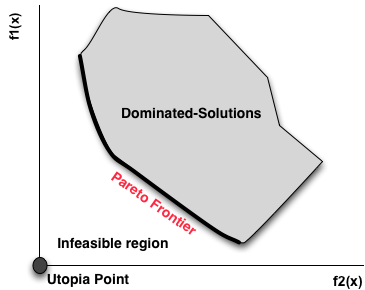
\includegraphics[width=0.4\textwidth]{./images/paretofront.png}
\caption{An mimization pareto front example}
\label{fig:pareto1}
\end{figure}

What distinguishes multi-objective EAs from singleobjective metaheuristics is how they rank and select individuals in the population. If there is only one objective, individuals are naturally ranked according to this objective, and it is clear which individuals are best and should be selected as
parents. In case of multiple objectives, it is still necessary to rank the individuals, but it is no longer obvious how to do this. Most people probably agree that a good approximation to the Pareto front is characterized by:

\begin{itemize}
\item  a small distance of the solutions to the true Pareto frontier,
\item  a wide range of solutions, i.e., an approximation
of the extreme values, and
\item a good distribution of solutions, i.e., an even
spread along the Pareto frontier.
\end{itemize}

Multi-objective metaheuristics rank individuals according to how much they contribute to the above goals.

The implementation adapted for this paper is based on the NSGA-II algorithm.  Deb et al.  proposed the NSGA II taking into account the need to reduce computational complexity in non-dominated classification, introduce elitism and eliminate subjectivity in the allocation of the sharing parameter \cite{Deb2000}. NSGA II (Non-dominated Sorting Genetic Algorithm II)  is a multiobjective algorithm, based on Genetic Algorithms  and that implements the concept of Dominance, that is, to classify the Total Population in fronts according to the degree of dominance. According to NSGA II, the individuals that are located on the first front are considered the best solutions of that generation, while in the last front are the worst. Using this concept, one can find more consistent results, points closer to the Pareto region, and that are better adapted to the type of problem. 

The NSGA algorithm II applies a fitness evaluation in an initial population (Figure \ref{fig:nsga2}- \ding{202} and \ding{203}). The population are ranked using multiple tournament selection, which consists of comparing two solutions (Figure \ref{fig:nsga2}- \ding{204}). In order to estimate the density of the solutions surrounding a particular solution in the population, the common distance between the previous solution and the posterior solution is calculated over each of the objectives. This distance serves as an estimate of the size of the largest cuboid that includes solution i without including any other solution of the population. A solution i wins another solution if:

\begin{itemize}
\item Solution i has a better rank, then $Rank_i$ <$Rank_j$.
\item Both solutions have the same rank, but i has a
Distance better than j, then $Rank_i$ = $Rank_j$ and $Distance_i$>$Distance_j$.
\end{itemize}

At the end of each analysis a certain group of individuals are classified as belonging to a specific category called the front and upon completion of the classification process all individuals will be inserted into one of the n fronts. Front 1 is made up of all non-dominated solutions. Front 2 can be achieved by considering all non-dominated solutions excluding solutions from front 1. For the determination of front 3, solutions previously classified on front 1 and 2 are excluded, and so on until all individuals have been Classified on some front.

After selection, recombination and mutation are performed as in conventional Genetic Algorithms (Figure \ref{fig:nsga2}- \ding{205}). The two sets (father and son of the same dimension) are united in a single population (dimension 2) and the classification is applied in dominance fronts. In this way, elitism is guaranteed preserving the best solutions (fronts not dominated) in the later population (Figure \ref{fig:nsga2}- \ding{207}).

However, not all fronts can be included in the new population. Thus, Deb et al. proposed a method called crowd distance , which combines the fronts not included in the set, to compose the last spaces of the current population, guaranteeing the diversity of the population \cite{Deb2000}. The NSGA-II algorithm creates a set of front lines, each front containing only non–dominating solutions. Within a front, individuals are rewarded for being ‘spread out’. The algorithm also ensures that the lowest ranked individual of a front still has a better fitness value than the highest ranked individual of the next front \cite{Harman2007}.




\begin{figure}[h]
\centering
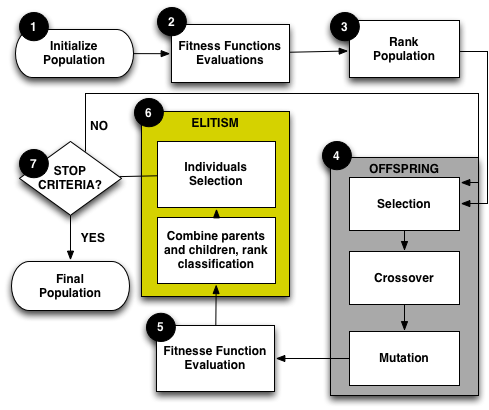
\includegraphics[width=0.5\textwidth]{./images/NSGA-2.png}
\caption{NSGA-II Algorithm}
\label{fig:nsga2}
\end{figure}

\FloatBarrier
\section{Search-based stress testing applications using NSGA-II }




The proposed solution makes it possible to create a model that perform search-based stress tests with  two distinct objectives. In the solution, each workload represent an individual in the search space. The solution implements the NSGA-II algorithm in IAdapter plugin. IAdapter is a JMeter plugin designed to perform search-based stress tests.  The plugin is available at \url{www.github.com/naubergois/newiadapter}.  The NSGA-II implementation used an adapted implementation of the jMetal framework (\url{http://jmetal.sourceforge.net/}). The next subsections present details about the solution life cycle, the solution representation, the crossover and mutant operators and the IAdapter Components. 

\subsection{Solution life cycle}

Figure. \ref{fig:step2} presents the proposed solution life cycle. Given an initial population (Figure \ref{fig:step2}  -\ding{202}),  the NSGA-II algorithm implementation receive a set of workloads  (Figure \ref{fig:step2}  -\ding{203}). The NSGA-II implementation generates a new set of individuals based on crossover or/and mutant operators (Figure \ref{fig:step2}  -\ding{204}).  JMeterEngine run each workload (Figure \ref{fig:step2}  -\ding{206}) and the NSGA-II algorithm ranks and classifies each workload based on objective functions  (Figure \ref{fig:step2}  -\ding{207}).  After all these steps the cycle begins until the maximum number of generations it is reached (Figure \ref{fig:step2}  -\ding{208}). 

\begin{figure}[h]

\centering
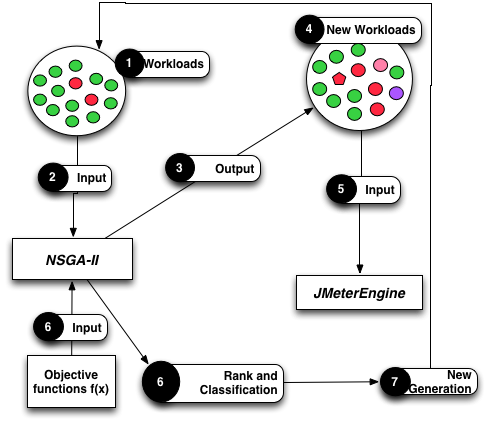
\includegraphics[width=0.5\textwidth]{./images/step3.png}
\caption{Test module life cycle.}
\label{fig:step2}

\end{figure} 

\subsection{Solution representation}

Figure. \ref{fig:solution} presents the solution representation and an example using the crossover operation. In the example, solution 1 (Figure \ref{fig:solution}  -\ding{204}) has the Login scenario with 2 users, the Search scenario with 4 users, Include scenario with 1 user and the Delete scenario with 2 users.  After the crossover operation with solution 2 (Figure \ref{fig:solution}  -\ding{205}), We obtain a solution with the Login scenario with 2 users, the Search scenario with 4 users, the Update scenario with 3 users and the Include scenario with 5 users (Figure \ref{fig:solution}  -\ding{206}). Figure. \ref{fig:solution} -\ding{207} shows the strategy used by the proposed solution to  obtain the neighbors for the Tabu search and simulated annealing algorithms. The neighbors are obtained by the modification of a single position (scenario or number of users) in the vector.


\begin{figure}[h]
\centering
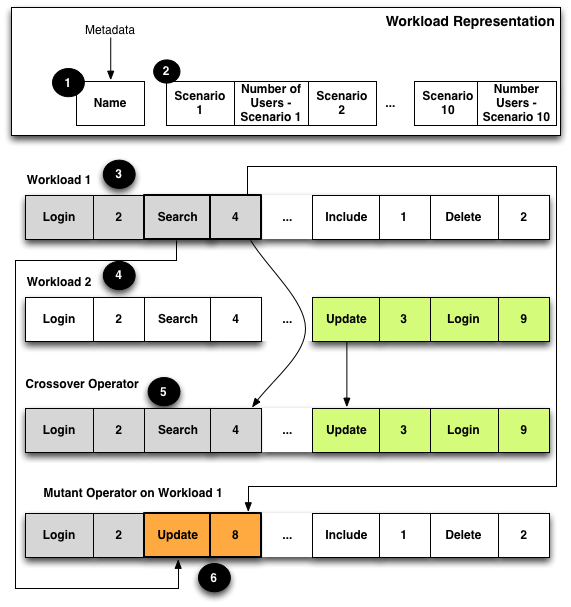
\includegraphics[width=0.5\textwidth]{./images/genomere.png}
\caption{Solution representation, crossover  and mutant operators}
\label{fig:solution}
\end{figure}



\subsection{IAdapter Components}
 
WorkLoadThreadGroup is a component that creates an initial population and configures the algorithms used in IAdapter. Fig. \ref{fig:tela1iadapter} presents the main screen of the WorkLoadThreadGroup component. The component has a name \ding{202}, a set of configuration tabs \ding{203}, a list of individuals by generation \ding{204}, a button to generate an initial population \ding{205}, and a button to export the results \ding{206}.

WorkLoadThreadGroup component uses the GeneticAlgorithm, TabuSearch and SimulateAnnealing classes.  The WorkLoadSaver component is responsible for saving all data in the database. The operation of the component only requires its inclusion in the test script.

WorkLoadController represents a scenario of the test. All actions necessary to test an application should be included in this component. All instances of the component need to login into the application under test and bring the application back to its original state.

\begin{figure}[h]
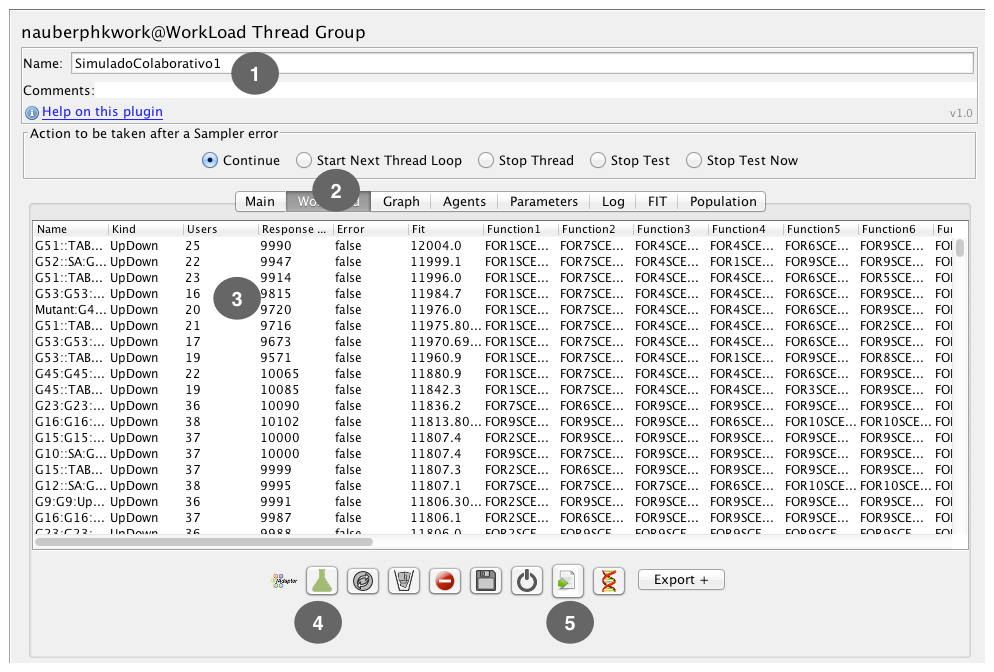
\includegraphics[width=0.5\textwidth]{./images/tela1iadapter.png}
\caption{WorkLoadThreadGroup component}
\label{fig:tela1iadapter}
\end{figure}

\section{Experimental Results}

In this section, We present the result of the experiment which we carried out to verify the multiobjective NSGA-II   implementation. The experiment was conducted to validate the use of NSGA-II multiobjective algorithm with a real implemented application. The chosen application was the JPetStore, available at \url{https://hub.docker.com/r/pocking/jpetstore/}. The maximum tolerated response time in the test was 500 seconds.  The whole process of stress  tests, which run for 3 days and 492 executions, was carried out without the need for monitoring by a test designer. The tool automatically selected the next scenarios to be run up to the limit of 123 generations previously established by algorithm. The experiments use the follow application features:


\begin{itemize}
\item Enter in the Catalog: the application presents the catalog of pets.
\item Fish: The application shows the recorded fish items.
\item Register:  a new user is registered into the system.
\item Dogs: The application shows the recorded dogs supplies.
\item Shopping Cart: the application displays the shopping cart.
\item Add or Remove in Shopping Cart: the application adds and removes items from shopping cart.
\end{itemize}

The experiments used an initial population of 4 individuals by metaheuristic. The genetic algorithm used the top 10 individuals from each generation in the crossover operation  The mutation operation was applied to 10\% of the population on each generation. The objective functions applied is intended to minimize the number of users and maximize the response time of the scenarios being tested. A penalty is applied when an application under test takes a longer time to respond than the maximum response time expected. 

The experiment used the following objective equations:

\begin{equation}
\begin{aligned}
objective function 1 =-3*numberOfUsers\\
-penalty\\
\end{aligned}
\end{equation}


\begin{equation}
\begin{aligned}
objective function 2 =responsetime\\
-penalty\\
\end{aligned}
\end{equation}

The first objective function seeks to find workloads with greater number of users and shorter response time. The second objective function seeks to find workloads with fewer users and longer response times. The penalty is calculated by the follow equation:

\begin{equation}
\begin{aligned}
penalty=100 * \Delta \\
\Delta=(t_{Current Response Time} - t_{Maximum Response Time Expected})\\
\end{aligned}
\end{equation}



\subsection{Experiment Research Questions}

The following research question is addressed:
\begin{itemize}
\item Does the NSGA-II algorithm find relevant workload scenarios according to the two test objectives?
\end{itemize}

\subsection{Variables}

The independent variable is the NSGA-II algorithm used in the test. The dependent variables are: the optimal workload scenario found by the algorithm.

\subsection{Hypotheses}

\begin{itemize}
\item With regard to multi-objectives applied in the experiment:
\begin{itemize}
\item $H_{0}$ (A null hypothesis) :The NSGA-II doesn't found workloads that meet the two objective functions used in the experiment.
\item $H_{1}$  : The NSGA-II  algorithm found workloads that meet the two objective functions used in the experiment.
\end{itemize}
\end{itemize}

\subsection{Results}

Fig. \ref{fig:paretofrontier1} and Table \ref{tab:results} present the results obtained in the experiment. The experiment found 9 optimal workloads (Pareto Frontier) that present a lower number of users with high response times. The workload number 1 with a single user accessing the dog scenario presented the response time of 245 seconds.  The workload number 2 with a single user accessing the dog scenario, 7 users accessing the Enter Catalog feature and 3 users in register functionality presented the response time of 400 seconds.



\begin{figure}[h]
\centering
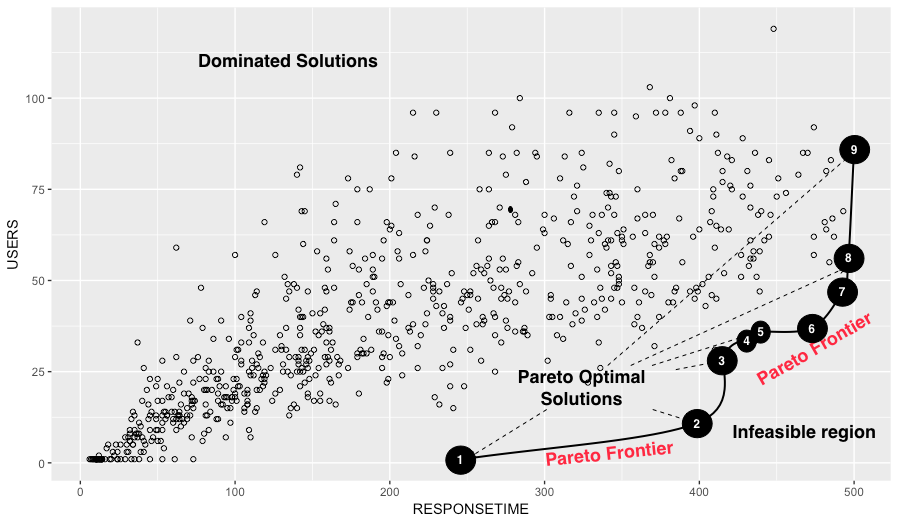
\includegraphics[width=0.5\textwidth]{./images/pareto0curve.png}
    \caption{Experiment Pareto Frontier}
\label{fig:paretofrontier1}
\end{figure}

% Please add the following required packages to your document preamble:
% \usepackage[table,xcdraw]{xcolor}
% If you use beamer only pass "xcolor=table" option, i.e. \documentclass[xcolor=table]{beamer}
\begin{table}[]
\centering
\caption{Pareto Frontier workloads results}
\label{tab:results}
\begin{tabular}{|l|l|l|l|l|l|l|l|l|}
\hline
\rowcolor[HTML]{C0C0C0} 
\textbf{N.} & \textbf{\begin{tabular}[c]{@{}l@{}}OBJ.\\ 1\end{tabular}} & \textbf{\begin{tabular}[c]{@{}l@{}}OBJ. \\ 2\end{tabular}} & \multicolumn{1}{c|}{\cellcolor[HTML]{C0C0C0}\textbf{\begin{tabular}[c]{@{}c@{}}Dogs\\ Users\end{tabular}}} & \textbf{\begin{tabular}[c]{@{}l@{}}Enter\\ Catalog\\ Users\end{tabular}} & \textbf{\begin{tabular}[c]{@{}l@{}}Fish\\ Users\end{tabular}} & \textbf{\begin{tabular}[c]{@{}l@{}}Register\\ Users\end{tabular}} & \textbf{\begin{tabular}[c]{@{}l@{}}Add\\ Rem.\\ Cart\end{tabular}} & \textbf{\begin{tabular}[c]{@{}l@{}}Cart\\ Users\end{tabular}} \\ \hline
\ding{202}           & -3                                                        & 245                                                        & 1                                                          &                                                                  &               &                   &                                                                    &               \\ \hline
\ding{203}           & -33                                                       & 400                                                        & 1                                                          & 7                                                                &               & 3                 &                                                                    &               \\ \hline
\ding{204}           & -87                                                       & 416                                                        & 5                                                          & 15                                                               & 4             & 5                 &                                                                    &               \\ \hline
\ding{205}          & -102                                                      & 434                                                        & 16                                                         & 17                                                               &               &                   &                                                                    & 1             \\ \hline
\ding{206}           & -105                                                      & 436                                                        & 15                                                         & 4                                                                & 8             & 3                 & 5                                                                  &               \\ \hline
\ding{207}           & -111                                                      & 472                                                        & 7                                                          & 13                                                               & 7             & 3                 & 7                                                                  &               \\ \hline
\ding{208}           & -141                                                      & 493                                                        & 7                                                          & 11                                                               & 11            & 7                 & 7                                                                  & 4             \\ \hline
\ding{209}           & -112                                                      & 496                                                        & 6                                                          &                                                                  & 12            & 8                 & 19                                                                 & 9             \\ \hline
\ding{210}           & -255                                                      & 499                                                        &                                                            & 54                                                               & 12            &                   & 7                                                                  & 12            \\ \hline
\end{tabular}
\end{table}


\subsection{Threats to validity}
\begin{itemize}
\item Construct Validity: 
In this work, we just evaluate the use of one multiobjective algorithm. However, several multiobjective algorithms could be applied.  There is still a reasonable distance between the Pareto frontier and the data obtained for the second objective, and more experiments are needed to validate the results.
\item Conclusion Validity: 
The workloads found by NSGA-II may be the result of the elitist strategy used in the algorithm that can be applied in the genetic algorithm.
\end{itemize}
% conference papers do not normally have an appendix

% use section* for acknowledgment
\section{Conclusion}


The experiment verified the use of an multi-objective algorithm in search-based stress testing problem. A tool named IAdapter, a JMeter plugin for performing search-based load tests, was extended.  One experiment was conducted to validate the proposed approach. The experiment use NSGA-II algorithm to discover application scenarios where there is a high response time for a small number of users. The whole process of stress  tests, which run for 3 days and 492 executions, was carried out without the need for monitoring by a test designer.  The experiment found 9 optimal workloads that present a lower number of users with high response times. The results of the experiment can help in the decision making of the service levels to be defined for the application. Future works intend to research the use of other algorithms such as SPEA2, PAES, PESA-II.





% trigger a \newpage just before the given reference
% number - used to balance the columns on the last page
% adjust value as needed - may need to be readjusted if
% the document is modified later
%\IEEEtriggeratref{8}
% The "triggered" command can be changed if desired:
%\IEEEtriggercmd{\enlargethispage{-5in}}

% references section

% can use a bibliography generated by BibTeX as a .bbl file
% BibTeX documentation can be easily obtained at:
% http://mirror.ctan.org/biblio/bibtex/contrib/doc/
% The IEEEtran BibTeX style support page is at:
% http://www.michaelshell.org/tex/ieeetran/bibtex/
%\bibliographystyle{IEEEtran}
% argument is your BibTeX string definitions and bibliography database(s)
%\bibliography{IEEEabrv,../bib/paper}
%
% <OR> manually copy in the resultant .bbl file
% set second argument of \begin to the number of references
% (used to reserve space for the reference number labels box)


\FloatBarrier
\bibliographystyle{IEEEtran}
\bibliography{cit}




% that's all folks
\end{document}


